\normaltrue \difficilefalse \tdifficilefalse
\correctionfalse
%\UPSTIidClasse{11} % 11 sup, 12 spé
%\newcommand{\UPSTIidClasse}{11}

\exer{Banc hydraulique $\star$ \label{C2:03:prec:63} 
%% CCP MP 2010
\setcounter{numques}{0}
\UPSTIcompetence[2]{C2-03}
\index{Compétence C2-03}
\index{Schéma-blocs}
\index{Précision}

\ifcorrection
\else
\textbf{Pas de corrigé pour cet exercice.}
\fi



Pour limiter l’erreur statique due aux fuites, on envisage d’asservir la pression d’eau dans le tube. 
%L’objectif est ici de proposer un réglage du correcteur pour répondre aux critères du cahier des charges.
La pression d’eau à l’intérieur du tube est mesurée par un capteur de pression. 

\begin{center}
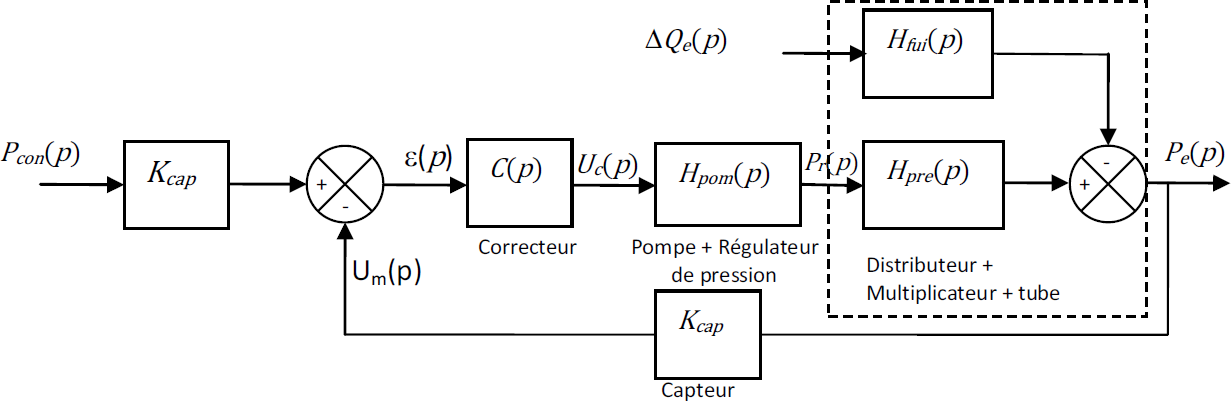
\includegraphics[width=\linewidth]{63_01}
\end{center}

 
 \begin{tabular}{ll}
$P_{\text{con}}(p)$ : & 	pression de consigne d’eau dans le tube (Pa) \\
$P_e(p)$ : & 	pression d’eau dans le tube (Pa) \\
$U_c(p)$ : & 	tension de commande du régulateur de pression (V)\\
$P_r(p)$ : &	pression d’huile régulée (Pa)\\
$\Delta Q_e(p)$ :& 	débit de fuite (\si{m^3s^{-1}})\\
$Um(p) 	:	tension de mesure du capteur (V)\\
\end{tabular}
 
 Hypothèses :
\begin{itemize}
\item Ll’ensemble de mise sous pression {tube + distributeur + multiplicateur de pression} est défini par les transmittances suivantes : $H_{\text{pre}} (p)=\dfrac{K_m}{1+T_1 p}$	et	$H_{\text{fui}} (p)=\dfrac{K_f}{1+T_1 p}$ avec 	$K_m = 3,24$ ; 	$K_f = \SI{2,55e10}{Pa.m^{-3}.s}$ ; 	$T_1  = \SI{10}{s}$.
\item L’ensemble {pompe+régulateur de pression} est modélisé par la fonction de transfert :
$H_{\text{pom}} (p)=\dfrac{K_{\text{pom}}}{1+T_2 p}$  avec 	$K_{\text{pom}} = \SI{1,234e7}{Pa/V}$; 	$T_2 = \SI{5}{s}$.
\item Le capteur est modélisé par un gain pur :	$K_{\text{cap}} = \SI{2,5.10e-8}{V/Pa}$.
\end{itemize}
La pression de consigne est de $P_{\text{con}} = \SI{800}{bars}$ et les débits de fuite sont estimés à $\Delta Q_e = \SU{5e-4}{m3/s}$.

 
Le cahier des charges concernant le réglage de la pression de test est le suivant.
\begin{center}
\begin{tabular}{ll}
\hline 
Stabilité :  & marge de phase de 60\degres  \\
  	  &  marge de gain de \SI{12}{dB} \\ \hline
Rapidité :  &  temps d’établissement te < 40 s \\ \hline
Précision : & 	erreur statique < 5\% soit pour une consigne de 800 bars : \\
&erreur statique due à la consigne : $\varepsilon_{\text{con}}< 5\%$  \\
& erreur statique due à la perturbation $\varepsilon_{\text{pert}} < \SI{40}{bars}$ \\ \hline
Amortissement :&	pas de dépassement \\ \hline
\end{tabular}
\end{center}

Dans le cas d’un système bouclé convenablement amorti, on pourra utiliser, sans aucune justification, la relation :
$t_e \cdot \omega_{\SI{0}{dB}}=3$ où $\omega_{\SI{0}{dB}}$ désigne la pulsation de coupure à \SI{0}{dB} en boucle ouverte et $t_e$ le temps d’établissement en boucle fermée vis-à-vis d’un échelon de consigne :
\begin{itemize}
\item $t_e = t_m$, temps du 1er maximum si le dépassement est supérieur à \SI{5}{\%},
\item $t_e = t_R$, temps de réponse à \SI{5}{\%} si le dépassement est nul ou inférieur à \SI{5}{\%}.
\end{itemize}
On envisage tout d’abord un correcteur de type proportionnel : $C(p)=K_p$. 

\question{Déterminer, en fonction de $K_p$ ,  $\varepsilon_{\text{con}}$ définie comme l’erreur statique pour une entrée consigne $P_{\text{con}}$ de type échelon, dans le cas où le débit de fuite est nul.}
\ifprof
\else 
\fi

\question{Proposer un réglage de $K_p$ pour limiter $\varepsilon_{\text{con}}$ à la valeur spécifiée dans le cahier des charges.}
\ifprof
\else 
\fi

\question{Dans le cas où la consigne de pression est nulle,  déterminer en fonction de $K_p$ la fonction de transfert en régulation définie par : $H_{\text{pert}}(p)=\dfrac{P_e (p)}{\Delta Q_e (p)}$. En déduire, en fonction de $K_p$,  $\varepsilon_{\text{pert}}$  définie comme l’erreur statique pour une perturbation $\Delta Q_e$ de type échelon, dans le cas où la consigne de pression est nulle.}
\ifprof
\else 
\fi

\question{Proposer un réglage de $K_p$ pour limiter $\varepsilon_{\text{pert}}$ à la valeur spécifiée au cahier des charges.}
\ifprof
\else 
\fi

\question{Proposer un réglage de $K_p$ pour vérifier le critère d’amortissement. Conclure quant au choix d’un correcteur proportionnel.}
\ifprof
\else 
\fi
 

\ifprof
\else

\noindent\footnotesize
\fbox{\parbox{.9\linewidth}{
Éléments de corrigé : 
\begin{enumerate}
  \item $\varepsilon_{\text{con \%}} = \dfrac{1}{1+K_PK_m K_{\text{pom}} K_{\text{cap}} }$;
  \item $K_P > 19$;
  \item $\varepsilon_{\text{pert}} = \Delta Q_e \dfrac{K_f}{1+K_{\text{cap}}K_PK_mK_{\text{pom}}}$;
  \item $K_P > 2,19$.
  \item $K_P < 0,125$. Il est impossible de vérifier les trois conditions avec un correcteur proportionnel.
\end{enumerate}}}
\normalsize

\begin{flushright}
\footnotesize{Corrigé  voir \ref{C2:03:prec:63}.}
\end{flushright}%
\fi